\documentclass{standalone}
% pdflatex tabular_data.tex
% magick -density 300 tabular_data.pdf -quality 90 -resize 640x640 tabular_data.png
\usepackage{tikz}
\usetikzlibrary{arrows.meta}

\begin{document}

% Statistical learning
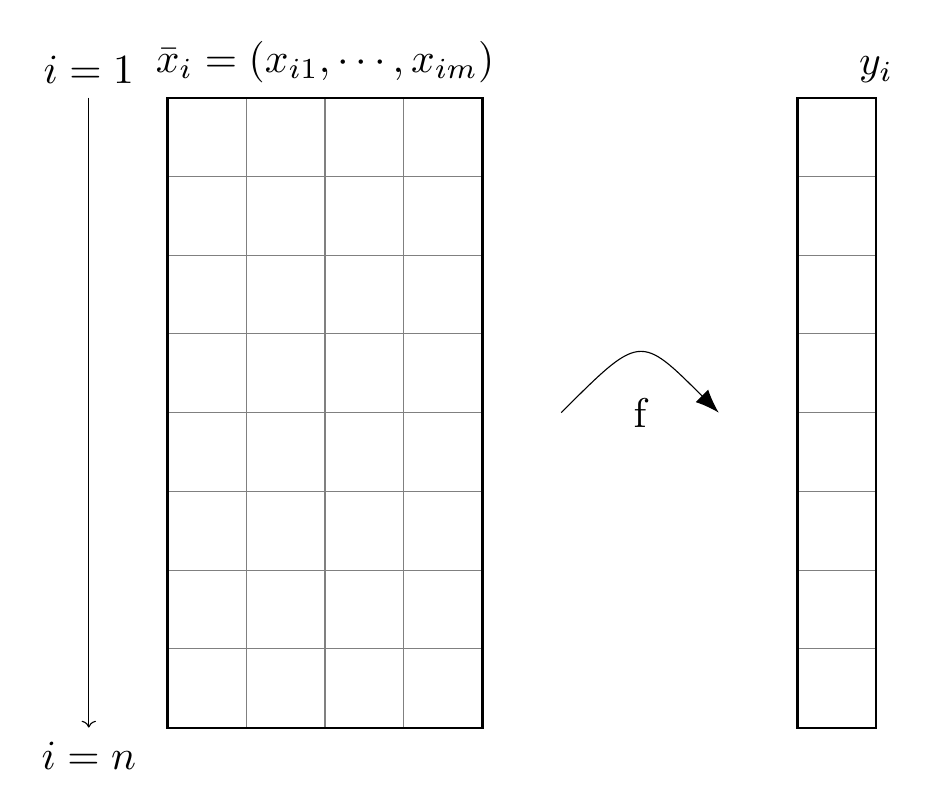
\begin{tikzpicture}

\draw[step=1cm,gray, thin] (0,0) grid (4,8);

\draw[thick, black] (0,0) rectangle (4,8);

\draw[black, ->]
   (-1,8) node[align=left, above, scale=1.5] {$i=1$}
-- (-1, 0) node[align=left, below, scale=1.5] {$i=n$};

\draw[-{Latex[length=3mm]}] (5,4) .. controls (6,5) ..  (7, 4);



\draw[step=1cm,gray, thin] (8,0) grid (9,8);
\draw[thick, black] (8,0) rectangle (9,8);

\node[scale=1.5]  at (6,4) (a1) {f};
\node[align=center, above, scale=1.5] at (2,8) (a2)  {$\bar{x}_i = (x_{i1}, \cdots, x_{im})$};
\node[align=left, above, scale=1.5]  at (9,8) (a3)  {$y_i$};

\end{tikzpicture}

\end{document}
